\section[RESTful WebService (Baris Akdag)]{RESTful WebService\begin{tiny} (Baris Akdag)\end{tiny}}
\subsection{Kommunikation}
Um die Kommunikation zwischen den Geräten zu ermöglichen, wird ein Internetdienst in Form eines \dq{}RESTful WebService\dq{} verwendet. \dq{}RESTful\dq{} steht dabei für \dq{}Representational State Transfer\dq{} und ist ein Programmierparadigma für Webanwendungen. Die Geräte können über den zentralen Dienst die Daten speichern und abfragen. Der RESTful WebService stellt alle notwendigen Funktionalitäten zur Geräteverwaltung, Erdbebenerkennung und Erdbebenwarnung zur Verfügung. 

\subsection{Grundlagen}
Bei einem \dq{}RESTful WebService\dq{} kommuniziert über das \dq{}Hypertext Transfer Protocol\dq{} (HTTP). Das hat den Vorteil, dass der Dienst programmiersprachenunabhängig integriert werden kann. Des Weiteren existieren durch den Einsatz von HTTP bereits viele fertige RESTful WebService Implementierungen, so dass diese relativ einfach in verschiedenen Applikationen benutzt werden können.

\parskip 12pt
Bei einem RESTful WebService wird mit Ressourcen gearbeitet. Die Ressourcen werden als \dq{}Uniform Resource Locator\dq{} (URL) dargestellt, dies ist umgangssprachlich eine Internetadresse der Form \dq{}http://www.name.com/pfad/ort\dq{}. Dabei ist in diesem Beispiel \dq{}/pfad/ort\dq{} die anzufragende Ressource. Es gibt verschiedene Befehle für spezifische Funktionen.


\subsubsection{GET}
Der Befehl \textbf{GET} wird verwendet um eine angegebene Ressource vom Server anzufordern. GET weist keine Nebeneffekte auf, da es nur lesend auf die Ressource zugreift, deshalb wird GET als sicher bezeichnet. Das folgende Beispiel ruft beispielsweise die Ressource \dq{}/itp/device/g52t\dq{} auf.

\begin{lstlisting}[caption={Beispiel HTTP GET Anfrage bei RESTful WebServices}]
GET http://www.it-projekt.de/itp/device/g52t HTTP/1.1
\end{lstlisting} 

Eine Antwort auf die GET Anfrage könnte beispielsweise das Registrierungsdatum des Geräts zurückgeben.

\begin{lstlisting}[caption={Beispiel Antwort auf die HTTP GET Anfrage}]
HTTP/1.1 200 OK
Date: Wed, 08 Jan 2014 19:33:21 GMT
Content-Type: application/json

{"registration":"2014-01-08","success":true}
\end{lstlisting} 

\subsubsection{POST}
Um Daten auf dem Zielsystem zu verändern wird der Befehl \textbf{POST} benutzt. POST kann Nebeneffekte aufweisen, da es Daten verändert und damit auch Daten unwiderruflich zerstören kann. Der POST Befehl wird daher als unsicher bezeichnet. Im folgenden Beispiel wird in der Ressource \dq{}/itp/register/g52t/date/2014-02-10\dq{} das Datum \dq{}2014-02-10\dq{} für das Gerät \dq{}g52t\dq{} gespeichert.

\begin{lstlisting}[caption={Beispiel HTTP GET Anfrage bei RESTful WebServices}]
POST http://www.it-projekt.de/itp/register/g52t/date/2014-02-10 HTTP/1.1
\end{lstlisting} 

Die Antwort auf die POST Anfrage könnte zurückgeben, ob die Daten erfolgreich gespeichert wurden.

\begin{lstlisting}[caption={Beispiel Antwort auf die HTTP POST Anfrage}]
HTTP/1.1 200 OK
Date: Wed, 08 Jan 2014 19:33:21 GMT
Content-Type: application/json

{"success":true}
\end{lstlisting} 

\subsubsection{PUT}
Der Befehl \textbf{PUT} ist identisch mit dem Befehl POST, mit dem einzigen Unterscheid, dass dieser gewöhnlich genutzt wird, um Daten zu erzeugen. Ein neues Gerät mit der Nummer \dq{}h80z\dq{} kann mit PUT wie folgt erzeugt werden.

\begin{lstlisting}[caption={Beispiel HTTP PUT Anfrage bei RESTful WebServices}]
PUT http://www.it-projekt.de/itp/register/h80z HTTP/1.1
\end{lstlisting} 

Der Dienst könnte zurückgeben, dass das Gerät mit der Nummer \dq{}g52t\dq{} erfolgreich erstellt wurde.

\begin{lstlisting}[caption={Beispiel Antwort auf die HTTP PUT Anfrage}]
HTTP/1.1 200 OK
Date: Wed, 08 Jan 2014 19:33:21 GMT
Content-Type: application/json

{"success":true}
\end{lstlisting} 

\subsubsection{DELETE}
Damit Daten gelöscht werden können, wird der Befehl \textbf{DELETE} verwendet. Der Befehl sollte daher mit Vorsicht freigegeben werden. DELETE wird als unsicher bezeichnet. Um das Gerät mit der Nummer \dq{}g52t\dq{} zu löschen, wird folgende Anfrage an den RESTful WebService gestellt.

\begin{lstlisting}[caption={Beispiel HTTP DELETE Anfrage bei RESTful WebServices}]
DELETE http://www.it-projekt.de/itp/register/g52t HTTP/1.1
\end{lstlisting} 

Eine erfolgreiche Löschung des Geräts kann der Dienst mit folgender Antwort bestätigen.

\begin{lstlisting}[caption={Beispiel Antwort auf die HTTP DELETE Anfrage}]
HTTP/1.1 200 OK
Date: Wed, 08 Jan 2014 19:33:21 GMT
Content-Type: application/json

{"success":true}
\end{lstlisting} 

\subsection{Technologien}
Für die Entwicklung des RESTful WebServices für die Erdbebenerkennung wurden Standard-Bibliotheken als Basis benutzt. Diese bieten bereits stabile Funktionalitäten, um einen RESTful WebService zu realisieren. Folgende Technologien wurden eingesetzt.


\textbf{Java} wurde als Programmiersprache eingesetzt. Zur Implementierung eines RESTful WebServices in Java wurde die Standard-Bibliothek \textbf{JAX-RS} verwendet. JAX-RS hat den Vorteil, dass durch Annotationen von Methoden, diese als RESTful WebService bereitgestellt werden können. Die Bibliothek wird als eine JAR-Datei bereitgestellt und kann in das Eclipse-Projekt eingebunden werden, so dass die Funktionalität zur Verfügung steht. Des Weiteren ist die JAX-RS Bibliothek mit unter 50 Kilobyte sehr kompakt und arbeitet effizient. JAX-RS bietet lediglich die Bereitstellung von Methoden als RESTful WebService, benötigt jedoch einen separaten Webserver. Ein kleiner Webserver für RESTful Webservices ist \textbf{Jersey}. Jersey wird ebenfalls als eine JAR-Datei in das Eclipse-Projekt eingebunden, so dass man den Webserver von Java aus starten kann. Der Webserver bietet parallele Zugriffe auf einen WebService und genügt damit den Anforderungen des Projekts. Um die Daten zu speichern, wurde eine relationale Datenbank verwendet. Wichtige Kriterien bei der Auswahl der Datenbank waren, dass diese plattformunabhängig und ohne eigenen Server läuft, d. h. von Java aus direkt verwendet werden kann. Die Datenbank \textbf{H2} hat sich dabei als geeignet herausgestellt, da H2 komplett in Java geschrieben und damit plattformunabhängig ist. Ebenfalls benötigt H2 keinen Server, sondern kann über die eingebundene JAR-Datei im Projekt direkt auf die Datenbank zugreifen. Das weitverbreitete SQLite wurde nicht benutzt, da es in C geschrieben ist, um somit je nach 32-/64-Bit eingebunden werden muss. Der WebService gibt als Antwort immer ein JSON zurück. JSON ist ein Format, das aus der Programmiersprache JavaScript entstanden ist. Heutzutage wird es jedoch in nahezu allen gängigen Programmiersprachen unterstützt und dient besonders zum Serialisieren und Transportierten von Daten zwischen verschiedenen Applikationen bzw. Diensten. Als JSON-Bibliothek wurde die \textbf{GSON} verwendet, welche von Google bereitgestellt wird.


\subsection{Funktionalitäten}
Der Dienst muss verschiedene Funktionen für die Android Applikation und die Erdbebenerkennung bereitstellen. Im WebService wird mit Geokoordinaten gearbeitet. Die Geokoordinaten werden im Dezimalformat abgebildet. Jeder Punkt auf der Erde definierbar und wird mit der Breite (latitude) und Länge (longitude) dargestellt. Die Länge verläuft senkrecht auf Äquator und durch die Pole der Erde. Der Äquator ist Breite 0 und die Länge 0 ist einheitlich  definiert. Die nördliche Breite vom Äquator ist positiv, südliche Breite negativ. 

Es wurden einheitliche Parameter im WebService definiert. Dabei ist \textbf{\{identifier\}} die Identifikationsnummer des Geräts. Die Parameter \textbf{\{longitude\}} und \textbf{\{latitude\}} sind die Geokoordinaten Länge und Breite. Als Rückgabeformat dient ebenfalls eine einheitliche JSON-Struktur, die wie folgt aufgebaut ist:

\begin{lstlisting}[caption={Einheitliche Rückgabe JSON-Struktur}]
{
   "message":"",
   "data":"",
   "success":true
}
\end{lstlisting} 


Das Feld \textbf{message} wird mit einem Fehlertext befüllt, falls ein Fehler auftritt. Wenn kein Fehler aufgetreten ist, ist das Feld leer. In \textbf{data} werden Nutzdaten übertragen, die für die Anfrage relevant sind. Das Feld \textbf{success} gibt \textit{true} bei einer erfolgreichen Anfrage und \textit{false} bei einer fehlgeschlagenen zurück. Folgende Funktionen sind im WebService implementiert.

\textit{(1)} Ein Gerät wird mit der Identifikationsnummer und den Geokoordinaten (Breite und Länge) registriert. Dabei werden in der Datenbank der Aktivitätszeitstempel und die Geokoordinaten aktualisiert. Wenn eine Identifikationsnummer bereits vorhanden ist, wird diese mit den entsprechenden Daten überschrieben. In der Rückgabe wird bestätigt, dass die Registrierung durchgeführt wurde.

\begin{table}[!htb] 
    \begin{tabular}{l|l}
    \textbf{Befehl}    & PUT                                          \\ \hline
    \textbf{Ressource} & itp/device/register/\{identifier\}/\{latitude\}/\{longitude\} \\ 
    \end{tabular}
\end{table}

\begin{lstlisting}[caption={Rückgabe}]
{
   "message":"",
   "data":"",
   "success":true
}
\end{lstlisting} 


\textit{(2)} Alle registrierten und aktiven Geräte können zurückgeben werden. Wenn der Aktivitätsstempel eine Geräts neuer ist als 15 Minunten, wird das Gerät mit in die Liste der aktiven Geräte aufgenommen. Anderenfalls wird es nicht berücksichtigt. In der Rückgabe werden alle aktiven Geräte mit Identifikationsnummer, letzte Geokoordinaten und der Aktivitätszeitstempel in einer Liste zurückgegeben.

\begin{table}[!htb] 
    \begin{tabular}{l|l}
    \textbf{Befehl}    & GET                                          \\ \hline
    \textbf{Ressource} & itp/device/list \\ 
    \end{tabular}
\end{table}

\begin{lstlisting}[caption={Rückgabe}]
{
"message":"",
"data":[
{        
  "identifier":"spKbisL7Zo",
  "longitude":10.999259,
  "latitude":49.5629328,
  "activity":"2014-01-08 20:12:18"
}],
"success":true
}
\end{lstlisting} 

\textit{(3)} Ein Gerät kann mit der eigenen Identifikationsnummer und den Geokoordinaten einen Alarm am WebService melden. Das Gerät meldet einen Alarm, wenn es ein Erdbeben erkannt hat. Die Rückgabe bestätigt lediglich den gemeldeten Alarm.

\begin{table}[!htb] 
    \begin{tabular}{l|l}
    \textbf{Befehl}    & PUT                                          \\ \hline
    \textbf{Ressource} & itp/device/alarm/\{identifier\}/\{latitude\}/\{longitude\} \\ 
    \end{tabular}
\end{table}

\begin{lstlisting}[caption={Rückgabe}]
{
   "message":"",
   "data":"",
   "success":true
}
\end{lstlisting} 


\textit{(4)} Die Informationen zu den letzten 15 Erdbeben, die Anzahl der in den letzten 15 Minuten aktiven Geräte und die Version des WebServices werden zurückgeben. Die Rückgabe enthält alle genannten Daten in verschiedenen Listen.

\begin{table}[!htb] 
    \begin{tabular}{l|l}
    \textbf{Befehl}    & GET                                          \\ \hline
    \textbf{Ressource} & itp/device/meta \\ 
    \end{tabular}
\end{table}

\begin{lstlisting}[caption={Rückgabe}]
{"message":"", "data":{
      "connectedDevices":2,
      "earthquakes":[
         {
            "longitude":10.7128923,
            "latitude":49.6720895,
            "activity":"2014-01-08 18:47:27.149",
            "radius":150.0,
            "devices":2,
            "ratio":0.5
         }
      ],
      "version":"0.0.8"
   },
   "success":true
}

\end{lstlisting} 

\textit{(5)} Des Weiteren ist es möglich zu einer konkreten Identifikationsnummer die aktuellen Geokoordinaten und den Aktivitätszeitstempel des Geräts zurückgeben.

\begin{table}[!htb] 
    \begin{tabular}{l|l}
    \textbf{Befehl}    & GET                                          \\ \hline
    \textbf{Ressource} & itp/device/meta/\{identifier\} \\ 
    \end{tabular}
\end{table}

\begin{lstlisting}[caption={Rückgabe}]
{
   "message":"",
   "data":{
      "identifier":"spKbisL7Zo",
      "longitude":10.7266746,
      "latitude":49.6749456,
      "activity":"2014-01-08 20:45:50.899"
   },
   "success":true
}
\end{lstlisting} 

\textit{(6)} Bei jedem Aufruf der \textbf{Alarm} Methode wird automatisch diese Methode intern mit den an die Alaram Methode übergebenen Geokoordinaten aufgerufen. Die Methode analysiert Erdbeben in einem festgelegten Radius und verschickt bei einem erkannten Erdbeben Warnungen an alle aktiven Geräte. Die Rückgabe definiert lediglich den erfolgreichen Aufruf. Informationen, ob und wie ein Erdbeben erkannt wurde, werden in der Debug Methode angezeigt.

\begin{table}[!htb] 
    \begin{tabular}{l|l}
    \textbf{Befehl}    & POST                                          \\ \hline
    \textbf{Ressource} & itp/device/analyze/\{latitude\}/\{longitude\} \\ 
    \end{tabular}
\end{table}

\begin{lstlisting}[caption={Rückgabe}]
{
   "message":"",
   "data":"",
   "success":true
}
\end{lstlisting} 

\textit{(7)} Informationen zu erkannten Erdbeben und verschickten Benachrichtungen können mit dieser Methode als HTML angezeigt werden. Dadurch kann die Methode im Internet-Browser aufgerufen und betrachtet werden.

\begin{table}[!htb] 
    \begin{tabular}{l|l}
    \textbf{Befehl}    & GET                                          \\ \hline
    \textbf{Ressource} & itp/device/debug \\ 
    \end{tabular}
\end{table}

\begin{lstlisting}[caption={Rückgabe als HTML}]
2014-02-08 09:55:31 | METHOD | algorithm | searchDistance [km] | 150 | notifyDistance [km] | 300 2014-02-08 09:55:31 | METHOD | algorithm | notifyTimeout [s] | 900 | detectionRatio [%] | 0.5
2014-02-08 09:55:31 | METHOD | analyze | current ratio | 0.0 | notify devices | 0 
2014-02-08 09:55:31 | METHOD | analyze | updated notifies | false | saved earthquake | false
2014-02-08 10:11:57 | METHOD | Register | APA91bHRhAE1Mf8hymU7SjLs | 49.4521089 | 11.0921879
\end{lstlisting} 


\subsection{Datenbank}
Für die Realisierung des RESTful WebServices werden drei Tabellen benötigt. Die Datenhaltung der Gerätedaten wird in der Tabelle \textit{DEVICE} abgebildet. Die Tabelle \textit{EARTHQUAKE} speichert erkannte Erdbeben. In der Tabelle \textit{NOTIFICATION} werden die gemeldeten Alarme der Geräte gespeichert.


\begin{figure}[H]
\centering
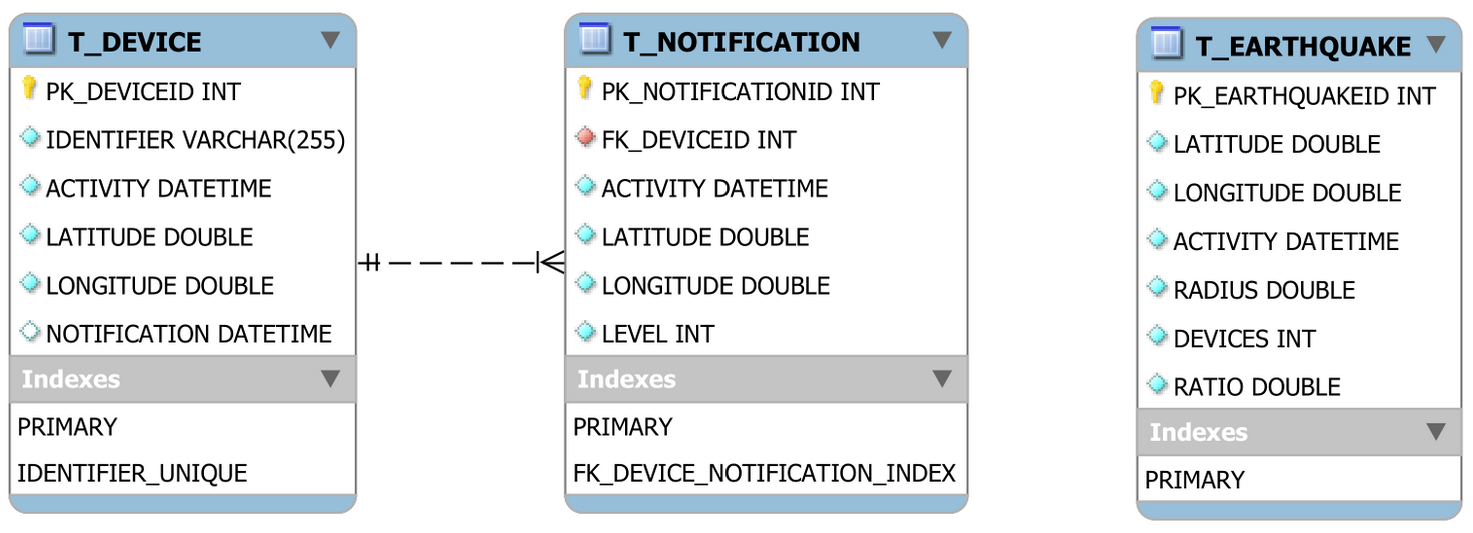
\includegraphics[width=16cm]{/ws-db.png}
\caption{Datenbankschema.}
\label{fig:WSDB}
\end{figure}

In der Tabelle \textbf{DEVICE} wird der Primärschlüssel (\textit{DEVICEID}), die Identifikationsnummer (\textit{IDENTIFIER}), der Aktivitätszeitstempel (\textit{ACTIVITY}), die Geokoordinaten Breite (\textit{LATITUDE}) und Länge (\textit{LONTITUDE}) und der Zeitstempel des letzten Benachrichtigung des Geräts gespeichert.

Die \textbf{NOTIFICATION} Tabelle enthält den Primärschlüssel (\textit{NOTIFICATIONID}), einen Fremdschlüssel zum registrierten Gerät (\textit{DEVICEID}), den Benachrichtigungszeitstempel (\textit{ACTIVITY}), die Geokoordinaten Breite (\textit{LATITUDE}) und Länge (\textit{LONTITUDE}). Das Feld (\textit{LEVEL}) war zur Einstufung der Erdbebenmeldung vorgesehen, wird jedoch zur Zeit nicht verwendet.

Die erkannten Erdbeben werden in der Tabelle \textbf{EARTHQUAKE} mit dem den Primärschlüssel (\textit{EARTHQUAKEID}) gespeichert. Des Weiteren werden benötigt: Die Geokoordinaten Breite (\textit{LATITUDE}) und Länge (\textit{LATITUDE}), den Zeitstempel des erkannten Erdbebens (\textit{ACTIVITY}), den verwendeten Suchradius des Erdbeben (\textit{RADIUS}), die zu dem Zeitpunkt aktive Geräteanzahl (\textit{DEVICES}) und der Prozentsatz wie viele Geräte zu diesem Erdbeben einen Alarm gemeldet haben (\textit{RATIO}).

Alle entsprechenden Fremdschlüssel zwischen den Tabellen gesetzt.

\subsection{Implementierung}
\subsubsection{Struktur}
Bei der Implementierung wurde darauf geachtet, dass zu jeder Klasse ein Interface implementiert wird. Ein Interface hat den Vorteil, dass bei Softwaretests (\textit{Unit Tests}) das Objekt einfacher durch ein Test-Objekt (\textit{Mockup}) ersetzt werden kann. Alle Interfaces wurden in einem eigenen Java-Paket (\textit{com.th.nuernberg.itp.webservice.interfaces}) gruppiert. Klassen die lediglich Daten abbilden wurden in einem eigenen Java-Paket (\textit{com.th.nuernberg.itp.webservice.types}) gehalten.

\subsubsection{Konfiguration}
Der WebSerivce kann über eine Konfigurationsdatei (\textit{conf/webservice.conf}) eingestellt werden. Es können Parameter wie beispielsweise Port des WebServices, Pfad zur Datenbankdatei, Debugdatei und Konfiguration des Erdbebenerkennungsalgorithmus eingestellt werden.


\subsubsection{Webserver}
Der Webserver wird in Java gestartet. Dazu wird in der statischen \textit{main}-Methode der StartJerseyServer-Klasse (\textit{StartJerseyServer.java}) die \textit{start}-Methode des Jersey Servers aufgerufen. StartJerseyServer-Klasse ist der Startpunkt des WebServices. 

\begin{lstlisting}[caption={Starten des Jersey Webservers.}]
public class StartJerseyServer {
	public static void main(String[] args) throws IllegalArgumentException, IOException, ClassNotFoundException, SQLException {
		
		ILogging console = new ConsoleLogging();
		
		IConfiguration config = new FileConfiguration();
		config.load(Constants.Configuration);

		String host = config.get("WebService.Host");
		String path = config.get("WebService.Path");
		String port = config.get("WebService.Port");
		String url = "http://"+host+":"+port+"/"+path;
		
		HttpServer server = HttpServerFactory.create(url);
		server.start();
	}

}
\end{lstlisting} 

Die Klassen \textit{ConsoleLogging} und \textit{FileConfiguration} sowie deren Interfaces \textit{ILogging} und \textit{IConfiguration} sind eigene Typen um die Konfiguration und die Debug-Ausgabe des WebServices zu ermöglichen. \textit{FileConfiguration} liest die Konfigurationsdatei ein. \textit{ConsoleLogging} implementiert einen Loggingmechanismus. Mit der \textit{create}- und \textit{start}-Methode wird der Webserver gestartet.


\subsubsection{WebService}
Die Entwicklung einer Methode im RESTful WebService kann über Annotationen umgesetzt werden. Diese werden über die Methode einer Klasse geschrieben und konfiguriert. Der folgende Quellcodeabschnitt zeigt die konkrete Implementierung der \textit{list}-Methode des WebServices.

\begin{lstlisting}[caption={Implementierung der list-Methode.}]
	@GET
	@Path("list")
	public String list() {

		DeviceRepository repository = new DeviceRepository();
		repository.setPersister(this.persister);
		List<IDevice> deviceList = repository.getActiveDevices(this.config.get("DeviceTimeout"));
		repository.destroy();		
		
		this.log.write("METHOD", "List", true, deviceList.size());
		return JsonWebResponse.build(true, deviceList);
	}	
\end{lstlisting} 

Die Annotationen \textit{GET} und \textit{Path} definieren den RESTful Befehl sowie die Ressource der Methode im WebService. Die Klasse \textit{DeviceRepository} enthält Methoden um Daten zu ermitteln oder zu ändern, bspw. die verwendete \textit{getActiveDevices} Methode. Mit \textit{Integer.parseInt(this.config.get("Application.DeviceTimeout"))} wird aus der Konfigurationsdatei der eingestellte Aktivitätszeitlimit (in Sekunden) für ein Gerät ermittelt, bspw. 900 bzw. 15 Miunten. Wird nun die Methode \textit{repository.getActiveDevices} mit diesem Parameter aufgerufen, werden alle aktiven Geräte innerhalb den letzten 15 Minuten ermittelt. Anschließend wird der Vorgang in der Debugdatei festgehalten und die Rückgabe mit der \textit{JsonWebResponse.build} gebaut.

\subsection{Erdbebenerkennung}
\subsubsection{Unterscheidung}
Im Algorithmus der Erdbebenerkennung werden diverse Parameter berücksichtigt. Die Erkennung basiert auf den Daten in der \textit{Notification}-Tabelle. Die Tabelle enthält alle gemeldeten Erdbeben der Geräte. Der Algorithmus unterscheidet zwischen den Geräten, die einen Alarm gemeldet haben, die in der nahen Umgebung dieses gemeldeten Erdbebens (\textit{Suchradius}) und den Geräten die in ferner Umgebung des gemeldeten Erdbebens (\textit{Warnradius}) sind.

\begin{figure}[H]
\centering
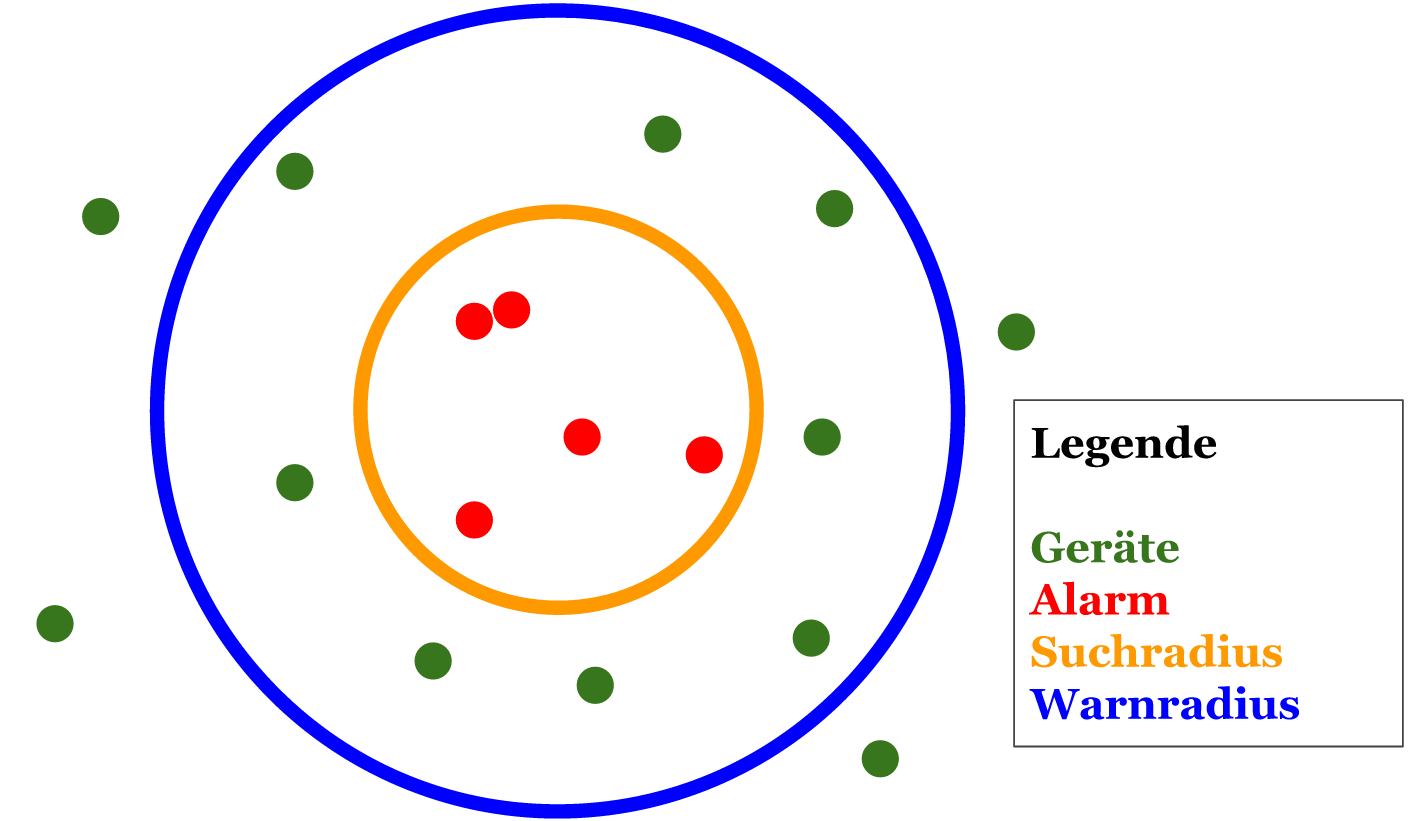
\includegraphics[width=16cm]{/ws-ee.png}
\caption{Erdbebenerkennung.}
\label{fig:WSEE}
\end{figure}

\subsubsection{Distanzberechnung}
Die Basis des Algorithmus ist die Berechnung zwischen zwei Geokoordinaten. Der Abstand zwischen zwei Geokoordinaten kann mit der sogannten \textit{Haversine}-Formel berechnet werden:

\begin{math}haversin(n) = sin2(n/2)\end{math}

\begin{math}a = haversin(\Delta latitude) + cos(latitude1) cos(latitude2) haversin(\Delta longitude)\end{math}

\begin{math}R = 6371 km\end{math}

\begin{math}distance = 2R atan(\sqrt{a}, \sqrt{(1-a))})\end{math}


Der Funktion werden zwei Geokoordinaten übergeben: \textit{latitude1} und \textit{latitude2}. \textit{R} definiert den Erdumfang in Kilometern, um die Distanz anschließend in Kilometern zu ermitteln.

\subsubsection{Algorithmus}
\textbf{Suchradius}: Das Erkennen eines Erdbebens wird in folgenden Schritten durchgeführt.

\begin{enumerate} 
\item Alle Geräte im Radius von 150 km ermitteln.
\item Einschränken auf Geräte, die in letzten 15 Minuten aktiv waren (devices). 
\item Ermitteln wie viele dieser Geräte einen Alarm gesendet haben (sent).
\item Prozentsatz: ratio = sent / devices
\end{enumerate}

\textbf{Warnradius}: Die zu benachrichtigenden Geräte werden wie folgt ermittelt.

\begin{enumerate} 
\item Alle Geräte im Radius von 300 km ermitteln.
\item Einschränke, die in letzten 15 min aktiv.
\item Prüfen, ob die letzte Benachrichtigung älter als 10 min ist.
\item Nach Versand letzte Benachrichtigung aktualisieren.
\end{enumerate}

Wenn der Prozentsatz in \textit{ratio} höher als ein definierter Wert in der Konfiguration ist, bspw. 66 Prozenz, wird ein Erdbeben erkannt und alle Geräte in der Nähe werden benachrichtigt. Erkannte Erdbeben werden anschließend zusätzlich in der Tabelle \textit{Earthquake} gespeichert.

\subsection{Benachrichtigung}
Die Benachrichtigung der Geräte bei einem Erdbeben wird über \textit{Google Cloud Messaging}  durchgeführt. Die Benachrichtigungen werden über einen sogenannte \textit{Push-Notifications} gesendet. Der Vorteil von Push-Notifications ist, dass das Gerät die Nachricht zugeschickt bekommt, wenn diese gesendet wurde. Dadurch muss das Gerät nicht permanent auf Nachrichten warten, sondern bekommt sie direkt zugestellt. Die Benachrichtigung eines Geräts erfolgt über die registrierte Identifikationsnummer, welche von Android bereitgestellt wird. 

Im WebService werden über den Google Cloud Messaging Dienst mit der URL \textit{android.googleapis.com/ gcm/send} die Nachrichten verschickt. Dafür wurden die Klasse \textit{GoogleCloudMessaging} und das passende Interface \textit{IGoogleCloudMessaging} implementiert. Die Klasse ermittelt baut aus allen übergebenen Identifikationsnummern eine HTTP Anfrage an das Google Cloud Messaging, so dass dieser umgehend die Nachrichten an die entsprechenden Geräte verschickt.

\subsection{Produktiveinsatz}
Der RESTful Webservice wurde zum Test auf den öffentlich erreichbaren Server mit der IP-Adresse \textbf{5.135.167.64} installiert. Dadurch kann der WebService jederzeit von der Android App benutzt werden, ohne den WebService lokal starten zu müssen. 

Der Server läuft unter einer Debian 7 64-Bit Distribution und Java 7. Obwohl der Server lediglich einen Zweikern Intel-Atom Prozessor und 2 GB Arbeitsspeicher besitzt läuft dieser relativ schnell und deckt die aktuellen Anforderungen der Erdbebenerkennung ab.